% ****** Start of file apssamp.tex ******
%
%   This file is part of the APS files in the REVTeX 4.2 distribution.
%   Version 4.2a of REVTeX, December 2014
%
%   Copyright (c) 2014 The American Physical Society.
%
%   See the REVTeX 4 README file for restrictions and more infor mation.
%
% TeX'ing this file requires that you have AMS-LaTeX 2.0 installed
% as well as the rest of the prerequisites for REVTeX 4.2
%
% See the REVTeX 4 README file
% It also requires running BibTeX. The commands are as follows:
%
%  1)  latex apssamp.tex
%  2)  bibtex apssamp
%  3)  latex apssamp.tex
%  4)  latex apssamp.tex
%
\documentclass[%
%  reprint,
%superscriptaddress,
%groupedaddress,
%unsortedaddress,
%runinaddress,
%frontmatterverbose, 
% preprint,
%preprintnumbers,
%nofootinbib,
%nobibnotes,
%bibnotes,
 amsmath,amssymb,
%  aps,
%pra,
% prb,
% rmp,
% prstab,
prstper,
% floatfix,
]{revtex4-2}

\usepackage[usenames, dvipsnames]{color}
% Color Edits
\newcommand{\EM}[1]{\noindent \color{red} (AA: #1)\normalcolor}
\newcommand{\AZ}[1]{\noindent \color{blue} (AZ: #1)\normalcolor}

\usepackage{braket}
\usepackage{graphicx}% Include figure files
\usepackage{dcolumn}% Align table columns on decimal point
\usepackage{bm}
\usepackage[usenames, dvipsnames]{color}
%\usepackage{hyperref}% add hypertext capabilities
%\usepackage[mathlines]{lineno}% Enable numbering of text and display math
%\linenumbers\relax % Commence numbering lines

%\usepackage[showframe,%Uncomment any one of the following lines to test 
%%scale=0.7, marginratio={1:1, 2:3}, ignoreall,% default settings
%%text={7in,10in},centering,
%%margin=1.5in,
%%total={6.5in,8.75in}, top=1.2in, left=0.9in, includefoot,
%%height=10in,a5paper,hmargin={3cm,0.8in},
%]{geometry}

\newcommand{\KB}[1]{\noindent \color{magenta} (KB: #1)\normalcolor}

\renewcommand{\thepage}{S\arabic{page}}
\renewcommand{\thesection}{S\arabic{section}}
\renewcommand{\thetable}{S\arabic{table}}
\renewcommand{\thefigure}{S\arabic{figure}}
\renewcommand{\theequation}{S\arabic{equation}}
\def\lp{\left(}
\def\rp{\right)}
\def\lb{\left[}
\def\rb{\right]}
\begin{document}


\preprint{APS/123-QED}



\title{Temporal Evolution of Flow in Pore-Networks:\\ From Homogenization to Instability}% Force line breaks with \\
% \thanks{A footnote to the article title}%

\author{Ahmad Zareei}
\affiliation{ School of Engineering and Applied Sciences, Harvard University, Cambridge, MA, 02148}%\altaffiliation[]{SEAS, Pierce Hall}%Lines break automatically or can be forced with \\
\author{Pan Deng}%
\affiliation{ School of Engineering and Applied Sciences, Harvard University, Cambridge, MA, 02148}%\altaffiliation[]{SEAS, Pierce Hall}%Lines break automatically or can be forced with
\author{Ariel Amir}%
\email{arielamir@seas.harvard.edu}
\affiliation{ School of Engineering and Applied Sciences, Harvard University, Cambridge, MA, 02148}%\altaffiliation[]{SEAS, Pierce Hall}%Lines break automatically or can be forced with
% need to figure out how to reference dagger




% \collaboration{MUSO Collaboration}%\noaffiliation

\date{\today}% It is always \today, today,
             %  but any date may be explicitly specified

\maketitle
\section{Simulation algorithm}
%
In our simulations, we tested two types of networks: (i) a topologically ordered (diamond-grid) network, (ii) a topologically random network (2d and 3d). 
% In the diamond-grid network, we choose 100 nodes in the horizontal direction $N_x=100$ and 50 nodes in the vertical direction $N_y=50$ which in total results in $20,000$ edges in the network (see \cite{githubrepo}). 
The 2d random network is created using uniformly distributed points with on average $N_x\times N_y$ nodes in the horizontal and vertical directions where the randomly distributed points are connected using a Delaunay triangulation. The 3d random network similarly is obtained by a uniform distribution of $N_x\times N_y \times N_z$ points in space, where the the points are connected using Voronoi cell initialization. The diameter of each edge is sampled from either a uniform distribution with $\mathcal{U}(1,14)$, log-normal distribution with $\mu=3,\sigma=0.48$, or truncated normal distribution with $\mathcal{N}(\mu=7.0,\sigma=3.6)$, where all of the distributions have a coefficient of variation close to $0.5$.  An external pressure is considered between the left-most nodes and the rightmost nodes ($p_\text{left}=10,p_\text{right}=0$). For each edge, assuming a Poiseuille flow, the fluid flux  $q$ and pressure difference $\delta P_e$ are related through $q_e = C_e \delta P_e$, where $C_e = \pi r^4_e/8\mu L_e$,  $L_e$ is the length of the tube, and $\mu$ is the viscosity of the fluid. We define $\vec{q}_e$ as the vector of fluid flux through all the edges, and as a result $\vec{q}_e = \mathbf{C} \mathbf{D}\vec{P}_n$ where $\vec{P}_n$ is the vector of pressure at all the nodes, $\mathbf{D}$ is the transpose of the network's oriented incidence matrix, and $\mathbf{C}$ is the diagonal matrix of edge conductances $\mathbf{C}_e = \text{diag} \left( C^{(1)}_e, C^{(2)}_e, \cdots,C^{(N_e)}_e\right)$. The orientation (or direction) of an edge is arbitrary selected, and it only determines the positive direction for the fluid flow in that edge. Next, we  use conservation of mass at the nodes to solve for the network pressure/flux at the nodes/edges. The conservation of mass at each node is 
%
\begin{align}
    \vec{q}_n = \mathbf{D}^\top \mathbf{C} \mathbf{D} \vec{P}_n, \label{eq:governeing}
\end{align}
%
where $\vec{q}_n$ is the vector of total incoming flow to each node. The total incoming flow to an internal node is zero inside the network due to the conservation of mass, and can only be non-zero at the boundary nodes. Without loss of generality, we renumber the boundary nodes to $1,2,\cdots, N_{B}$, where $N_B$ shows the total number of nodes at the boundary. We re-partition Eq. \eqref{eq:governeing} to obtain 

\begin{align}
 \begin{bmatrix} {\mathbf{D}_{b}}^\top \mathbf{C} {\mathbf{D}_{b}}  & \vline &    {\mathbf{D}_{b}}^\top \mathbf{C} {\mathbf{D}_{n}}\\ \hline   
    {\mathbf{D}_{n}}^\top \mathbf{C} {\mathbf{D}_{b}} & \vline & {\mathbf{D}_{n}}^\top \mathbf{C} {\mathbf{D}_{n}}
    \end{bmatrix} \begin{bmatrix} P^{BC}_1 \\ P^{BC}_2 \\ \vdots \\ P_{N_B} \\  \hline  P_{N_B+1} \\ \vdots \\ P_{N_n}
    \end{bmatrix} = \begin{bmatrix} q^{BC}_1 \\ q^{BC}_2 \\ \vdots \\ q^{BC}_{N_B} \\ \hline  0 \\ \vdots \\ 0\end{bmatrix} \to 
    \begin{bmatrix} 
    \mathbf{A}_{bb} & \mathbf{A}_{bn} \\
    \mathbf{A}_{nb} & \mathbf{A}_{nn}       
    \end{bmatrix} \begin{bmatrix} P^{BC}_1 \\ P^{BC}_2 \\ \vdots \\ P^{BC}_{N_B} \\ \hline  P_{N_B+1} \\ \vdots \\ P_{N_n}
    \end{bmatrix} = \begin{bmatrix} q^{BC}_1 \\ q^{BC}_2 \\ \vdots \\ q^{BC}_{N_B}  \\ \hline  0 \\ \vdots \\ 0\end{bmatrix}, 
\end{align}
%
where $\mathbf{A}_{st} = \mathbf{D}^\top_s \mathbf{C}\mathbf{D}^\top_t$ and  $s,t\in\left\{a,b\right\}$. The first $N_B$ elements of the pressure vector (i.e., $P_1, \cdots, P_{N_B}$) represent the pressure at the boundary nodes and the rest represent the pressure for the internal nodes. In summary the above equations can be written as a combination of two set of linear equations 
%
\begin{subequations}\label{main-solve-eq}
\begin{align}
%     \begin{cases} 
  & \mathbf{A}_{bb} \vec{P}_{BC} + \mathbf{A}_{bn}  \vec{P} = \vec{q}_{BC}, \label{maina} \\
& \mathbf{A}_{nb}\vec{P}_{BC} +  \mathbf{A}_{nn} \vec{P} = 0. \label{mainb}
%     \end{cases} 
    % \\ \mathbf{A}_{nn} \ket{P_n} =- \mathbf{A}_{nb}\ket{P_{BC}} 
    % \label{eq:main-network}
 \end{align}
\end{subequations}
%
where $\vec{P}_{BC} = [P^{BC}_1, \cdots, P^{BC}_{N_B}]^\top$ is the boundary nodes pressure vector, $\vec{q}_{BC} = [q^{BC}_1, \cdots, q^{BC}_{N_B}]^\top$ is the boundary nodes incoming fluid flux vector, and $\vec{P} = [P_{N_B+1}, \cdots, P_{N_n}]^\top$ is the unknown pressure vector for the rest of the nodes. If the pressure at the boundary is given,  we can use Eq. \eqref{mainb} to solve for the internal pressure values $\vec{P}$, and then use Eq. \eqref{maina} to find the required flux at the boundary nodes $\vec{q}_{BC}$. However, if fluid flux vector at the boundary nodes is given (i.e., $\vec{q}_{BC}$ is known), we need to simultaneously solve  Eqs. \eqref{maina} and \eqref{mainb} to find the boundary pressure vector  $\vec{P}_{BC}$ and internal nodes pressure vector $\vec{P}$. In either case, solving Eq. \eqref{main-solve-eq}  results in the nodes' pressure vector and also the fluid flux vector at the boundary nodes. The fluid flux at each edge can then be calculated using  $\vec{q}_e=\mathbf{C}_e \mathbf{D} \vec{P}_n$. Next, given the flux at each edge  $q_e$, we increase (decrease) the edge radius under erosion (clogging) using 
%
\begin{align}
    \frac{dr_e}{dt} \propto \pm  \frac{q^m_e}{r_e^n},
\end{align}
%
and re-iterate the process to solve for the new fluid flux vector. We use a simple forward Euler for time integration. For each iteration, we choose the time step $dt$ so that $\max(dr_e) = 0.1 r_0$, where $r_0$ is the smallest radius among all edges. 
% Note that $r_{ij} (t+\delta t)  = r_{ij} (t)  + (\alpha \delta t)  q_{ij} (t)/ r^n_{ij} (t) $, where the coefficient $\alpha \delta t$ is chosen such that the maximum change in the radius at each time step is smaller than one-tenth  of the smallest tube's radius i.e. $\max (\Delta r_{ij}) \leq r_\text{min}/10$ of the smallest radius at the initial configuration.  
This condition guarantees that at each step a small amount of material is eroded and there is no sudden change in the network. We further test the convergence by decreasing $\max(\Delta r_{ij})$ to half and we observe that the average relative change in the flux vector is $\approx 1.2\%$, and the PDFs remain intact without any notable change. The network size for the 2d/3d networks is $N_x=100,N_y=50$/$N_x=50,N_y=12, N_z=12$ unless mentioned otherwise. In either case, the network has an order of $10^3$ edges. The code is publicly available in a GitHub repository \cite{githubrepo}. 


%
% \begin{figure}[h]
%     % \centering
%     \includegraphics[width = 0.75\textwidth]{Figs/Fig2_random-low.png}
%     \caption{Ahmad's version: Erosion in a topologically random network of pipes. The first row shows the initial condition at $t=0$. Each row afterward corresponds to the simulation result after $N$ steps such that $\langle r_{t=N}\rangle=2r_0$ where $r_0 = \langle r_{t=0}\rangle$. The erosion law is based on Eq. (1) in the main text where different powers of $n$ correspond to different models of erosion. The first column is a snapshot of the pore network, the second column is the PDF of normalized fluid flux $q/\langle q \rangle$, and the last column is the PDF of normalized radius $r/\langle r\rangle$.}\label{fig:fig2}
% \end{figure}
%

\section{Analytical results for fluid flux EXP-tail PDF in a Diamond Network}
%
\label{sec:analytical}
%
As described in the main text, the PDF of flow in a topologically disordered network of tubes takes the same form  as in a  structured diamond grid. For completeness, here we repeat the derivation of Refs. \cite{liu1995force,coppersmith1996model,alim2017local} which  show that the observed exponential distribution of fluid flux can be described using a mean-field approach on a structured grid. Basically, the random distribution of the diameters along with the conservation of mass in the network are the two main ingredients resulting in an exponential tail distribution. In a diamond grid, the incoming flow to a node is redistributed among the outgoing edges (since fluid mass is conserved). Due to the randomness in the tube's diameter, the redistribution of the incoming flow to a node between the outgoing edges is random variable.  This model for the flow can be mapped one to one to the problem of force fluctuations in a bead pack \cite{liu1995force,coppersmith1996model,alim2017local} as shown in Fig. \ref{grid-result}. In a bead pack, the force at each layer is redistributed to the next layer where the total force exerted on the next layer should equal to that of the previous layer. 
%
\begin{figure}[h]
  \centering
  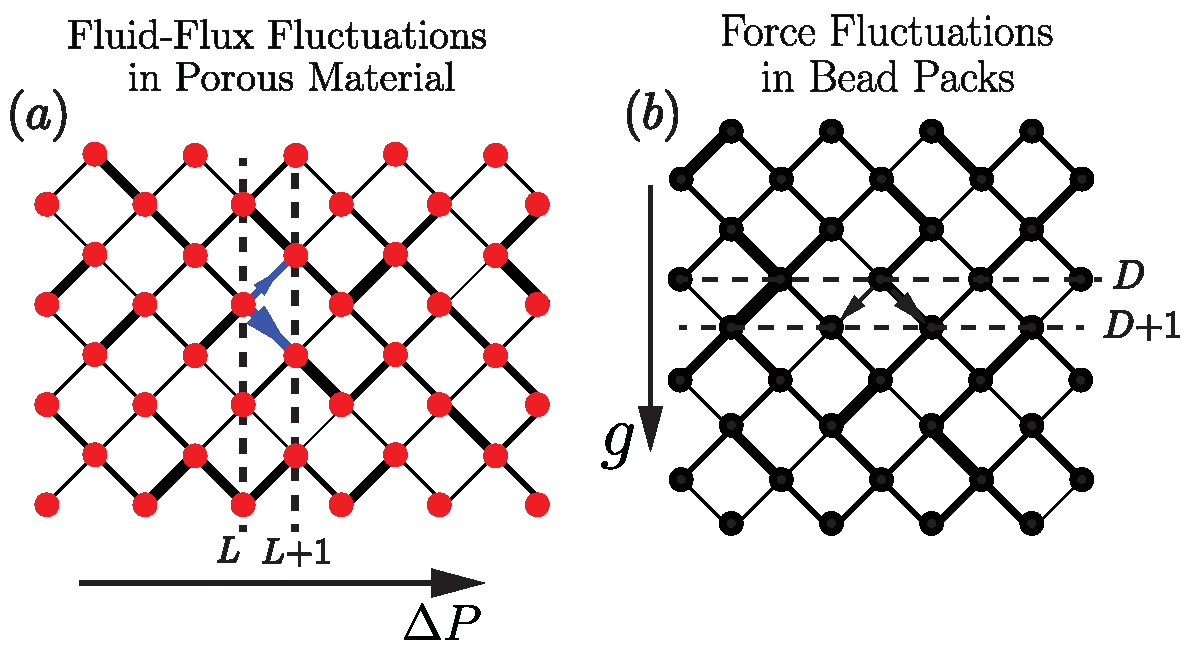
\includegraphics[width=.75\textwidth]{FigS1.pdf} % grid-analytica
  \caption{(a) Schematic of a  diamond grid network of tubes. The incoming flow to each node is redistributed among the outgoing edges. The thickness of the lines shows the fluid flux transferred through that edge. (b) Schematic diagram showing beads (represented with nodes) and their contacts to the neighboring sites (represented with edges). The thickness of the edges show the force transferred through that contact.} \label{grid-result}
\end{figure}
%
Given the above conditions, the flow at layer $L+1$ at node $j$ can be obtained as 
%
\begin{align}
  q(L+1,j) = \sum_i w_{ij} q(L,i) = w_{i,i+1} q(L,i+1) + w_{i,i} q(L,i), \label{total-flow}
\end{align}
%
where $w_{ij}$ shows the weights by which the flow is redistributed, and $\sum_{j} w_{ij} = 1$ since the total fluid flux is conserved. 
% Next, we assume that the weights $w_{ij}$ are drawn from a distribution $\eta(w)$. Since $\eta(w)$ is a distribution, then $\int \eta(w) dw = 1$. Furthermore, since $\sum_jw_{ij} = 1$, we can conclude that
%
%\begin{align}
%  \sum_j w_{ij}=1 \to N {E}[w_{ij}] = 1 \to E[w_{ij}] = 1/N \to {\int w\eta(w) dw = 1/N}
% \end{align}
%
Assuming a general distribution of for the weights, $\eta(w)$, we can use a mean-field approximation to find the distribution of $q$ at the layer $L$, i.e., $p_L(q)$, as 
%
\begin{align}
  p_L (q) = \prod_{j=1}^N \left\{ \int_0^1 d w_j \eta(w_j) \int_0^{\infty} dq_j p_{L-1}(q_j)\right\} \times \delta \left( \sum_j w_j q_{j} - q \right),
\end{align}
%
% The only approximation in the above equation is that we neglect the possible correlation between the values of $q$ among ancestors. 
where $N$ is the number of outgoing edges (e.g., in our structured diamond grid $N=2$) and $\delta(\cdot)$ is the Dirac delta function. 
% The constraint that $q$'s emanating downward should add up to one is accounted for through the definition of $\eta(w)$. 
% The values of flux at each layer $q(L,i)$ are not independent for neighboring sites; however, in our mean-field approximation, we ignore such correlations.  
Taking the Laplace transform of the above equation and defining $\tilde p(s)  \equiv \int_0^{\infty} p(q) e^{-qs} dq$ one obtains
%
% \begin{align}
 % \tilde P(s) & \equiv \int_0^{\infty} P(Q) e^{-Qs} dQ\\
%   \xrightarrow{\int_0^{\infty} (\cdot) e^{-Qs} dQ}  P (Q) & = \prod_{j=1}^N \left\{ \int_0^1 d w_j \eta(w_j) \int_0^{\infty} dQ_j P(Q_j)\right\} \times \delta \lp \sum_j w_j Q_{j} - Q \rp \\
%   \tilde P(s) & = \int_0^{\infty} \prod_{j=1}^N \left\{ \int_0^1 d w_j \eta(w_j) \int_0^{\infty} dQ_j P(Q_j)\right\} \times \delta \lp \sum_j w_j Q_{j} - Q \rp e^{-Qs}dQ \\
  %            & = \prod_{j=1}^N \left\{ \int_0^1 d w_j \eta(w_j) \int_0^{\infty} dQ_j e^{-\sum w_{j}Q_{j}} P(Q_j)\right\}   \\
%              & = \prod_{j=1}^N \left\{ \int_0^1 d w_j \eta(w_j) \tilde P(s w_j) \right\} \\
%   & = \lp  \int_0^1 d w \eta(w) \tilde P(s w)  \rp^{N}
% \end{align}
%
% Or in summary
%
\begin{align}
  {\tilde P_L(s) = \lp  \int_0^1 d w \eta(w) \tilde P_{L-1}(s w)  \rp^{N}}. \label{eq:main-laplace}
\end{align}
%
The above equation gives a recursive relation for the Laplace transformed of fluid flux PDF, $\tilde P_L(s)$, where it gradually converges to a distribution $\tilde P(s)$ from which the PDF of fluid flux can be obtained. Solving the above equation for a structured diamond grid network, one finds that the converged PDF of the fluid flux becomes $p(q) = 4q\exp(-2q)$ \cite{liu1995force,coppersmith1996model,alim2017local}, which is an exponential tailed distribution. 


% \begin{figure}[h]
    % \centering
%     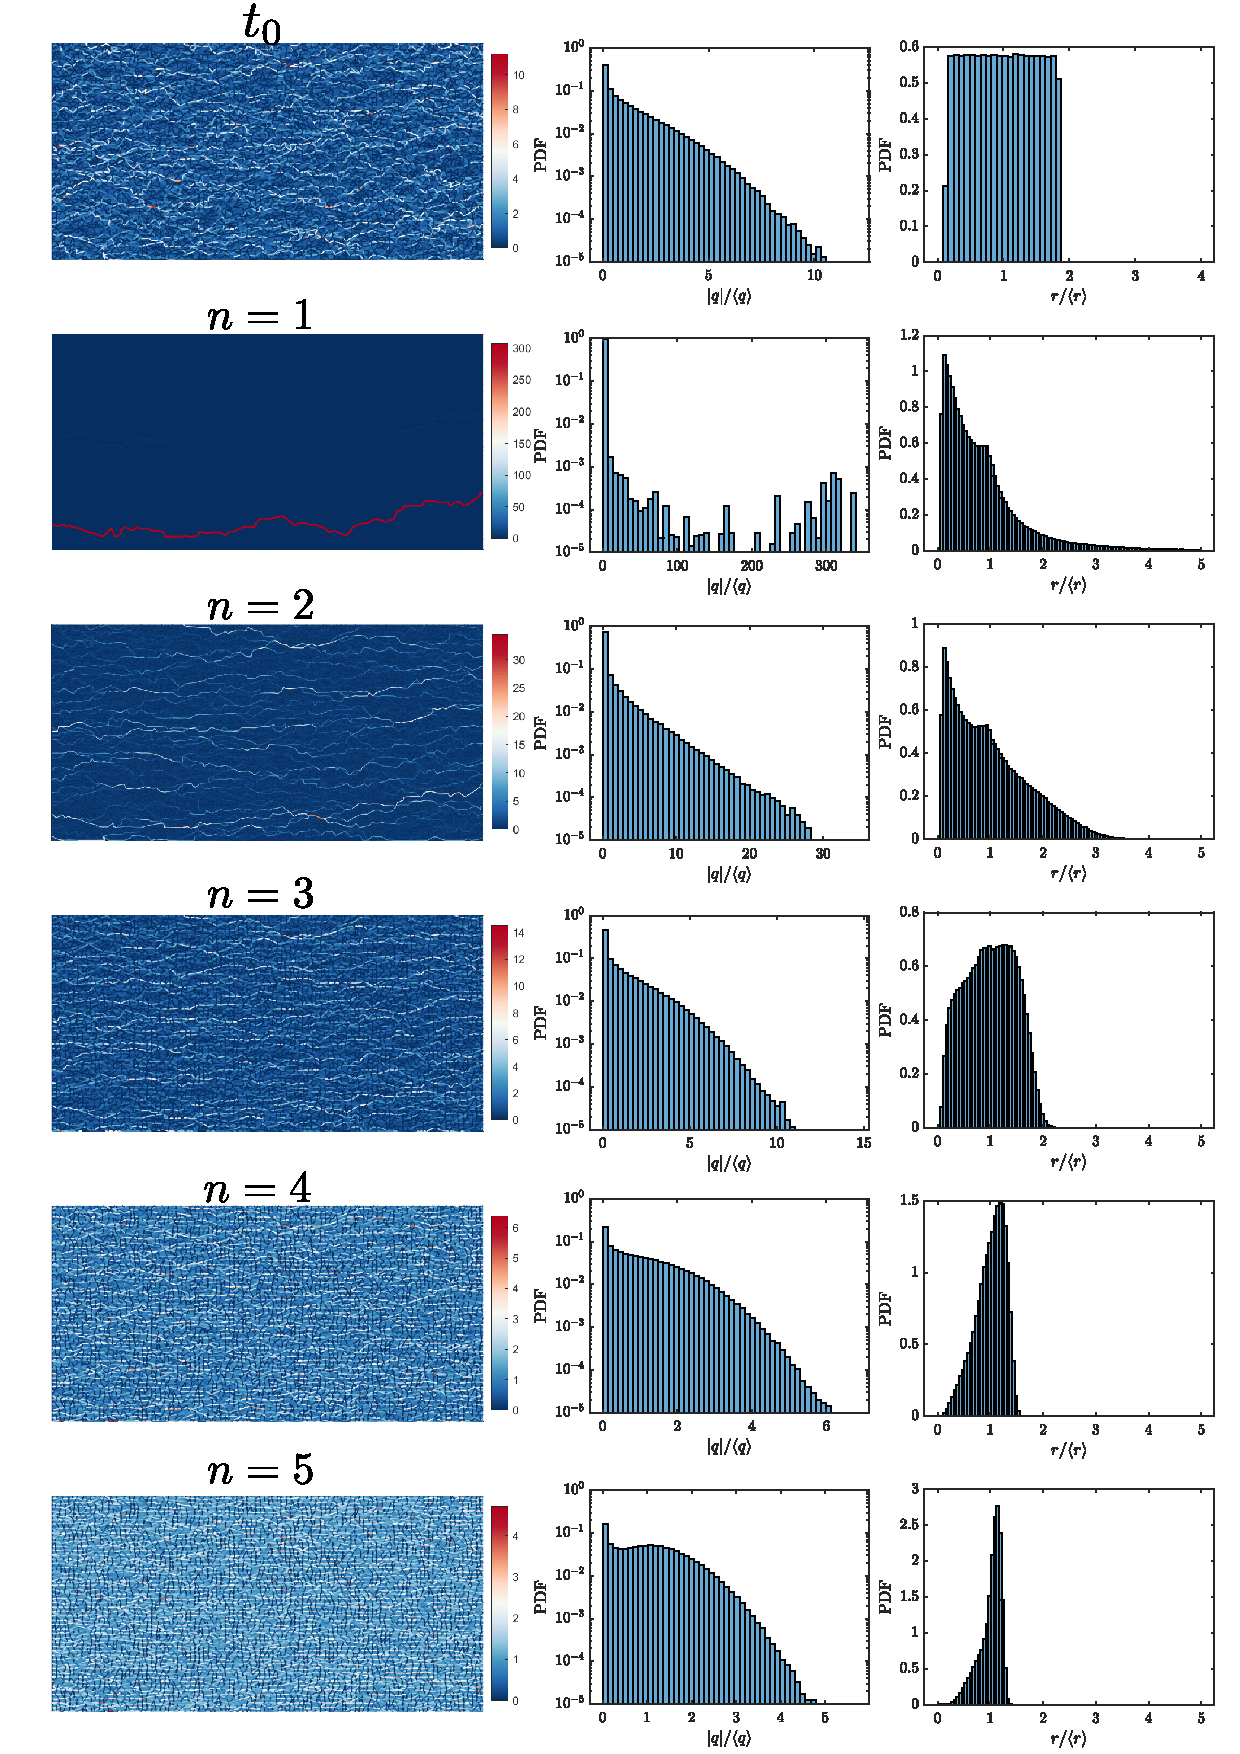
\includegraphics[width=0.75\textwidth]{Figs/randomNetworkErosion3.pdf}
%     \caption{Deng's version: Erosion in a topologically random network of pipes. The initial condition is shown with the label $t=0$ in the first row. Each row afterward corresponds to the simulation result after $N$ steps such that $\langle r_{t=N}\rangle=2r_0$ where $r_0 = \langle r_{t=0}\rangle$ or twice the initial average radius. The erosion law is based on Eq. (1) in the main text where different powers of $n$ correspond to different models of erosion. The first column is a snapshot of the pore network, the second column is the PDF of normalized fluid flux $q/\langle q \rangle$, and the last column is the PDF of normalized radius $r/\langle r\rangle$.}\label{fig:fig2}% 
% \end{figure}






\newpage
\section{Robustness to topology and initial condition}
% 
In order to check the robustness of our result with respect to the topology of the network, we run our simulations on a three-dimensional random network with Voronoi cell initialization of nodes in space (Fig. \ref{SIfig:fig2-3d}), and also for a two dimensional topologically ordered network with a diamond grid (Fig. \ref{fig:fig2-diamond}), where  both networks are initialized with a uniform random distribution for the diameter of the tubes. We find that regardless of the topology of the network, an erosion dynamics with $n>3$ results in a homogenized network, while $n<3$ results in the channelization instability. We further check the effect of initial randomness on the fate of the network. We use a two-dimensional diamond-grid network with a narrow uniform initial distribution of tube diameters around an average diameter $d_0$ with only a very small variation ($3\%$), i.e., the tube diameters are sampled from $\mathcal{U}(d_0(1-\epsilon), d_0(1+\epsilon))$. We again find that for the networks with $n<3$ channels are formed, while for $n>3$ the network stays homogenized.  
%
\begin{figure}[htp]
     % \centering
      \includegraphics[width = 1.0\textwidth]{FigS2.pdf}
     \caption{Erosion in a topologically random 3D network of tubes with $N_x=20, N_y=12, N_z=12$ points for Voronoi cell initialization and an initial uniform broad distribution of tube diameters randomly sampled from $\mathcal{U}(1,14)$. Snapshots of the network, PDF of normalized fluid flux $q/\langle q \rangle$, and normalized edge radius distribution $r/\langle r \rangle$ at the initial time $t=0$, and also after $N$ erosion steps for different powers of erosion $n$ are shown. We stop the erosion after $N$ steps such that $\langle r\rangle=2r_0$ where $r_0 = \langle r_{t=0}\rangle$. The erosion law is based on Eq. (1) in the main text where different powers of $n$ correspond to different models of erosion.}\label{SIfig:fig2-3d}
 \end{figure}
%
\begin{figure}[htp]
    % \centering
 \includegraphics[width=0.75\textwidth]{FigS3.pdf} % Fig2-Sdiamond.pdf
     \caption{Erosion in a diamond grid network with $N_x=100, N_y=50$ randomly distributed nodes and an initially broad  distribution of tube diameter randomly sampled from $\mathcal{U}(1,14)$. The initial condition is shown with the label $t=0$ in the first row. Each row afterward corresponds to the simulation result after $N$ steps such that $\langle r\rangle=2r_0$ where $r_0 = \langle r_{t=0}\rangle$ or twice the initial average radius. The erosion law is based on Eq. (1) in the main text where different powers of $n$ correspond to different models of erosion. The first column is a snapshot of the pore network, the second column is the PDF of normalized fluid flux $q/\langle q \rangle$, and the last column is the PDF of normalized radius $r/\langle r\rangle$.}\label{fig:fig2-diamond}% 
\end{figure}
%
\begin{figure}[htp]
    % \centering
 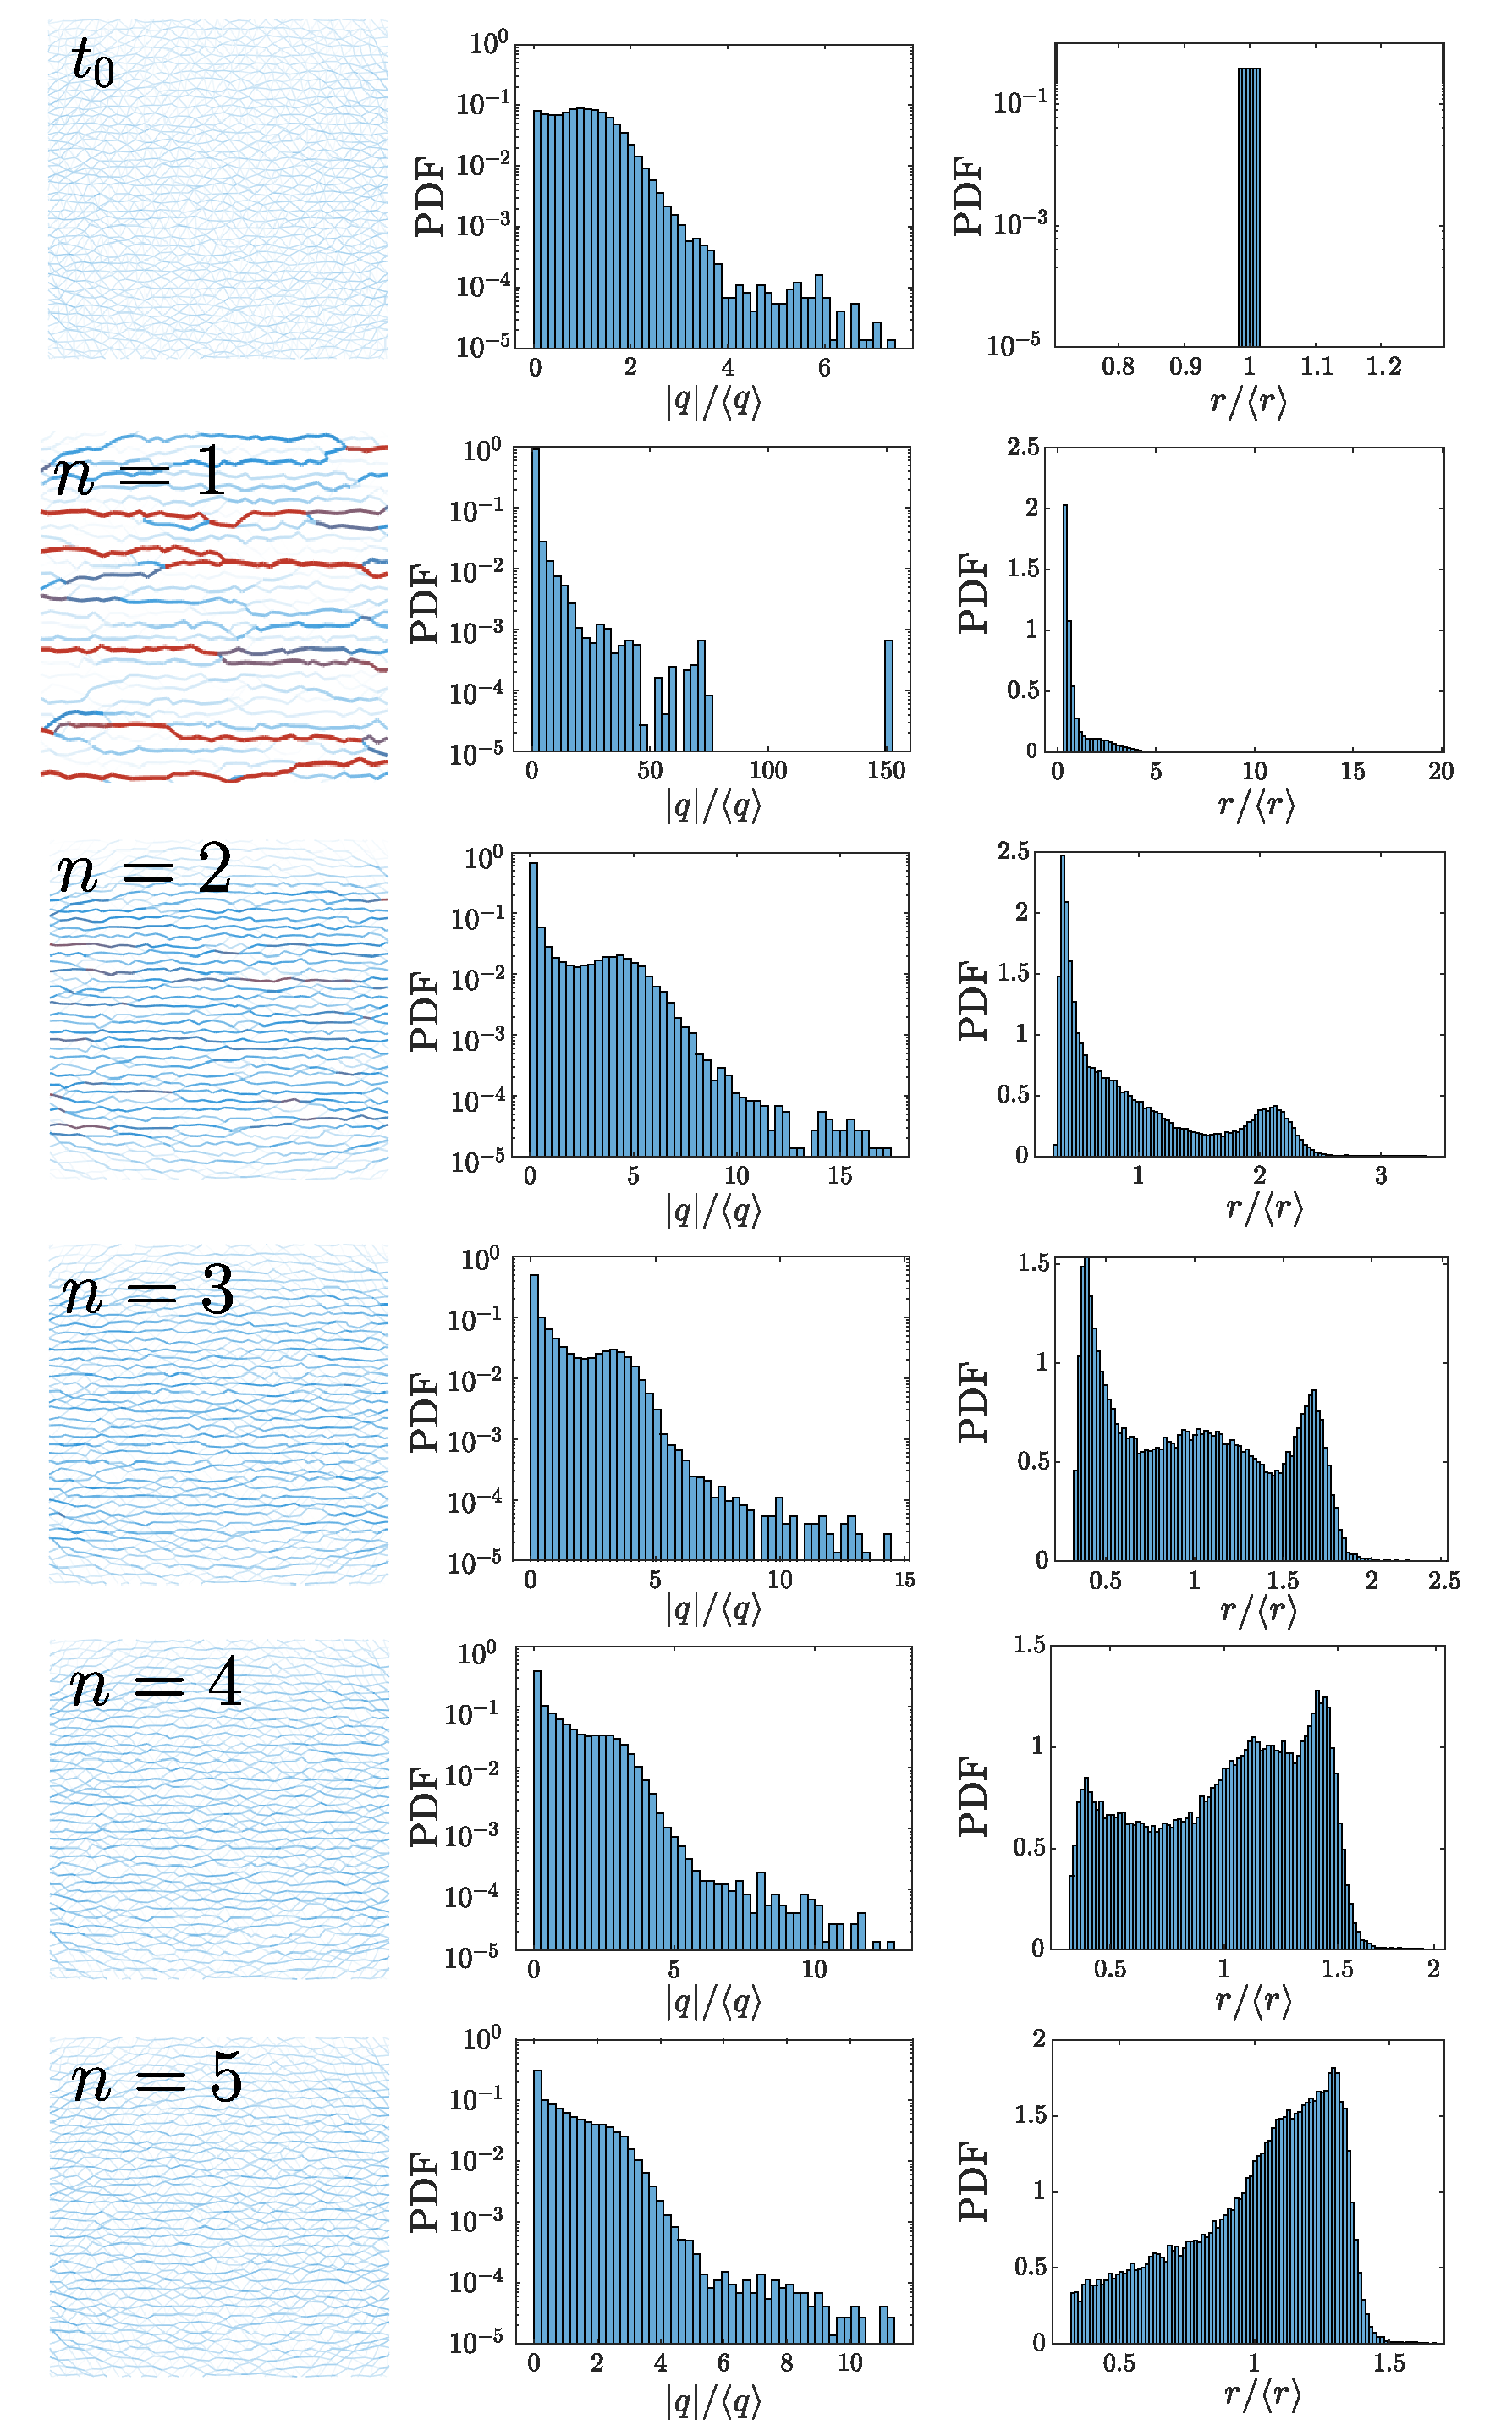
\includegraphics[width=0.72\textwidth]{FigS4.pdf}
     \caption{Erosion in a structured diamond grid network with $N_x=50, N_y=50$ and an initially narrow distribution of tube diameters randomly sampled from  $\mathcal{U}\left(d_0(1-\epsilon), d_u(1+\epsilon)\right) $ where  $d_0$ is the average diameter and $\epsilon=0.03$. The initial condition is shown with the label $t=0$ in the first row. Each row afterward corresponds to the simulation result after $N$ steps such that $\langle r_{t=N}\rangle=2r_0$ where $r_0 = \langle r_{t=0}\rangle$ or twice the initial average radius. The erosion law is based on Eq. (1) in the main text where different powers of $n$ correspond to different models of erosion. The first column is a snapshot of the pore network, the second column is the PDF of normalized fluid flux $q/\langle q \rangle$, and the last column is the PDF of normalized radius $r/\langle r\rangle$.}\label{fig:fig2}% 
\end{figure}




\newpage 
\newpage 
\newpage
\section{Average Change in the  Order parameter}
%
In order to quantify the network behavior shown in Fig. 4, we calculate the change in the order parameter for different $m,n$ averaged over 100 simulations with different random initial conditions, and the heat-map results are shown in Fig.~\ref{fig:fig4_SI-2}. The positive or negative change in the order parameter shows the network's change toward homogenization or channelization. The boundary between the two phases (homogenization and channelization) calculated using the simple model introduced in the main text is shown with a solid black line here, and it can be seen that it agrees well with the order parameter change. 
%
\begin{figure}[htp]
    % \centering
    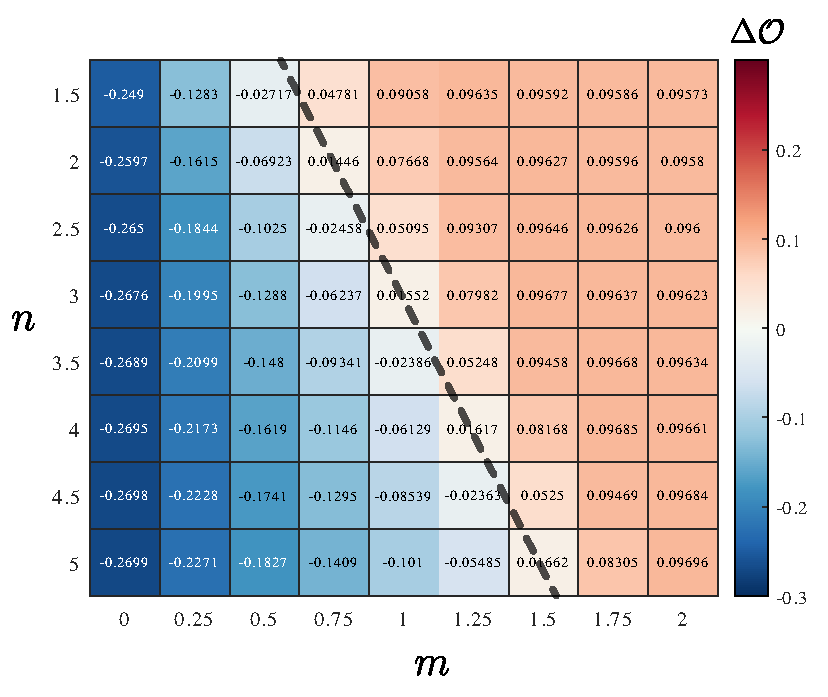
\includegraphics[width = 0.70\textwidth]{FigS5.pdf}
    \caption{The heat map for the average change in the order parameter corresponding to the networks shown in Fig. 4 of the main text. The order parameter shown in the heat map here is an average of 100 different simulations with different random initialization of tube diameters. The black line shows the boundary between two phases calculated using the model introduced in the main text.}\label{fig:fig4_SI-2}
\end{figure}




\section{Clogging Dynamics}
% 
% \textit{}-- 
Besides erosion, another change in the network is the deposition/sedimentation of material on the boundary walls of the porous material. We refer to this dynamical change a ``clogging'' process as opposed to erosion. Contrary to erosion, the clogging behavior may cause some edges to block which effectively alters the network of connectivity and network behavior. This change in the connection between nodes through edges getting blocked can drastically alter porous structure behavior, e.g., causes a huge difference between effective and true porosity \cite{shima2021}. Despite the drastic change of network with blockages, we can still focus on the \textit{initial} change in the order parameter. The derivative of order parameter can be written as 
%
\begin{align}
    \frac{d\mathcal{O}}{dt} = \sum_{ij} \sum_{kl} \frac{\partial \mathcal{O}}{\partial q_{ij}} \frac{\partial q_{ij}}{\partial C_{kl}}  \frac{\partial C_{kl}}{\partial t} \label{eq:order-derivative}
\end{align}
%
where the last term changes sign from erosion to clogging, i.e., $\partial C_{kl}/\partial t = \pm \alpha \pi q^m_{kl} /r_{kl}^{n-3}\mu l_{kl}$ for erosion and clogging respectively. As a result, the magnitude of change in the order parameter equals that of erosion. Note that in Eq. \eqref{eq:order-derivative}, the second term depends on the network topology, and pore throat clogging results in the change of network topology at later times.
% The pore throat blockages results in the divergent of clogging results from just the negative of erosion. 
At short times, however, similar to the erosion, a phase transition exists at $n=3$. When  $n<3$ the network moves toward homogenization during the clogging process and when $n>3$ the flow moves toward the development of channeling instability. At later times, this initial trend, however, might not hold true due to the aforementioned complex changes in the connectivity network during the clogging process. 



% \clearpage
\bibliography{ref}% Produces the bibliography via BibTeX.

\end{document}
%

%###############################################################
%###############################################################
%###############################################################
%###############################################################
%###############################################################
%###############################################################
%###############################################################


\newpage
\section{Clogging behavior at initial times}
% 
Considering a small change in the radius of edges, and as a result, the conductance of the edges $\mathbf{C}+\delta \mathbf{C}$, using Eq. \eqref{main-solve-eq} we find that 
%
\begin{align}
    \ket{P'} &=  \ket{P} -  \left( \Delta_n^\top\mathbf{C} \Delta_n\right)^{-1}\left[  \left( \Delta_n^\top \delta \mathbf{C} \Delta_n\right)\ket{P} + \left( \Delta_n^\top\delta \mathbf{C} \Delta_b\right) \ket{P_{BC}}\right],
\end{align}
%
where we used the fact that for an invertible matrix $\mathbf{A}$ we have 
%
\begin{align}
    \left(\mathbf{A} + \delta \mathbf{A} \right)^{-1} = \mathbf{A}^{-1} - \left( \mathbf{A}^{-1} \delta \mathbf{A}\right) \mathbf{A}^{-1} + \left( \mathbf{A}^{-1}  \delta \mathbf{A}\right)^{2}\mathbf{A}^{-1}  + \cdots.
\end{align}
%
Calculating for the changes in the fluid flux, we find that 
%
\begin{align}
\ket{q'} & = \left( \mathbf{C}+ \delta \mathbf{C}  \right)\left( \Delta_b \ket{P_{BC}} +  \Delta_n \ket{P'} \right) \\
& = \ket{q} + \delta\mathbf{C} \mathbf{C}^{-1}\ket{q} - \mathbf{C} \Delta_n \left( \Delta_n^\top\mathbf{C} \Delta_n\right)^{-1}\left[  \left( \Delta_n^\top \delta \mathbf{C} \Delta_n\right)\ket{P} + \left( \Delta_n^\top\delta \mathbf{C} \Delta_b\right) \ket{P_{BC}}\right].
\end{align}
%
The above equation can then be used to study the evolution of order parameter in the networks. Note that during the blockage of pore-throats, the connectivity between the nodes changes and as a result network's connectivity matrix $\Delta$ changes and the above approximation will not hold anymore.  

%###############################################################
%###############################################################
%###############################################################
%###############################################################
%###############################################################
%###############################################################
%###############################################################

% ****** End of file apssamp.tex ******

 If we set
$\eta(w) = \delta(w-1/2)$, then the flow at each node has probability of
$1/2$ to move to either of the neighboring sites. As a result the flow at a given depth $L$ will become homogeneous as $P_L(Q) = \delta (Q-\bar{Q})$ where $\bar{Q}$
is the average of input fluid flow. This results is the same as having the same
diameter for all the edges which results in a singular solution in the structured grid.
% 
\subsection*{$P(Q)$ decays faster than $Q^{-n}$ for any $n$}
We first show that $P(Q)$ decays faster than any power of $Q$ for any
weight distributions. We expand the Laplace transform using a Taylor expansion as 
%
\begin{align}
  \tilde P(s) = 1 + \sum_j \tilde P_{j} s^{j}.
\end{align}
%
Inserting this expansion into Eq. \eqref{eq:main-laplace}, we obtain
%
\begin{align}
  1 + \sum_j \tilde P_{j} s^{j}  & = \lp  \int_0^1 d w \eta(w) \lb 1 + \sum_j \tilde P_{j} (sw)^{j}\rb    \rp^{N}  = \lp  1 + \sum_j \tilde P_j \langle w^{j}\rangle  s^{j}   \rp^{N}
\end{align}
%
where $\langle w^j \rangle = \int_0^1 \eta(w) w^j dw$ is the $j$-th
moment of the weights $w$. In the above equation we can observe that
%
\begin{align}
  P_j \lp N \langle w^j\rangle -1 \rp = G(P_{j-1}, P_{j-1}, \cdots, P_1)
\end{align}
%
In the above equation $P_j$ can only diverge only if $N\langle w^j
\rangle -1=0$. If $w$ can only be zero and one, then $\langle
w^j\rangle =\langle w \rangle = 1/N$ and the coefficient can become
zero! Other than this special distribution, when $0 \leq w \leq 1$, then
%
\begin{align}
  & w\in [0,1] \rightarrow w>w^2>w^3> \cdots \\
  & \forall k>1 \rightarrow \langle w^k \rangle < \langle w \rangle = \frac{1}{N} 
\end{align}
%
which means that $N\langle w^j \rangle -1\neq 0$ and as a result
$P_j$ is finite. $P_j$ on the other hand is the $j$-th moment or
$\langle Q^j\rangle$ and it is finite. If $P\approx Q^{-n}$, then the
$n$-th moment will not be finite i.e. $\langle Q^{n+1}\rangle =
P_{n+1}$ is not finite. We can then conclude that $P(Q)$ should go to
zero faster than any $Q^{-n}$ as $Q\to \infty$! In other words $d \log
P(Q) / d \log Q \to -\infty$ as $Q\to \infty$.  
% 
\subsection*{Exponential Decay}
%
The main recursive governing equation for a diamond grid is  
%
\begin{align}
  \tilde P(s) = \lp  \int_0^1 d w \eta(w) \tilde P(s w)  \rp^{2} \label{eq:main-recur}
\end{align}
%
% In order to have an approximation for $\eta(w)$ we consider the following situation:
At each node there are two neighboring nodes where the flux is distributed by
$w_1$ and $w_2$ among them. Assuming that $w_1$ is uniformly distributed
between $0$ and $1$, then $w_2 = 1-w_1$ (due to  conservation of
mass $w_1 + w_2 = 1$). Now $\eta(w)$ can be obtained using 
%
\begin{align}
  & \eta(w) = M \int_0^1 dw_1 \delta(1-w_1-w) =  M, \\
  \text{since }& \int_0^1 \eta(w) dw = 1 \to M =1 \\
  & \eta (w) = 1
\end{align}
%
Just for completeness, if there are three neighboring connections ($N=3$), then we
have
%
\begin{align}
  \eta(w) & = M \int_0^1 dw_1 \int_0^1 dw_2 \delta(1-w_1-w_2 - w)\\
          & = M(1-w)  \to \int_0^1\eta(w) dw = 1 \to M = \frac{1}{2} \\
  & \eta(w) = \frac{1}{2} (1-w)
\end{align}
%
As a result Eq.~\eqref{eq:main-recur} simplifies to
%
\begin{align}
  \tilde P(s) = \lp  \int_0^1 d w  \tilde P(s w)  \rp^{2} 
\end{align}
%
In order to solve the above equation, we assume $\tilde V (s) =
\sqrt{\tilde{P}(s)}$.
%
\begin{align}
  \tilde{V}(s) & = \int_0^1 dw \tilde V (sw) = \int_0^s \frac{du}{s}  \tilde{V}^{2}(u) \\
  s\tilde{V}(s) & = \int_0^s du  \tilde{V}^2(u) \\
\end{align}
%
Taking the differentiation with respect to $s$ yields
%
\begin{align}
  \tilde{V}(s) + s \frac{d \tilde{V}(s)}{d s} = \tilde{V}^2(s) \\
  \frac{d \tilde{V}}{\tilde{V}^2-\tilde{V}} = \frac{ds}{s}  \\
  \log\lp \frac{1-\tilde{V}}{\tilde{V}} \rp  = \log(s)\\
  \tilde{V}(s) = \frac{1}{1+Cs} 
\end{align}
%
We set the mean to $1$ i.e.,
%
\begin{align}
  \int_0^{\infty} Q P(Q) dQ = 1 \to \frac{d\tilde{P}}{ds}|_{s=0}  = -1\\
  \frac{d \tilde{V}}{ds}  = \frac{1}{2 \sqrt{\tilde{P}(s)}} \frac{d \tilde{P}(s)}{d s}   \to \frac{d\tilde{V}(s)}{ds}|_{s=0} =\frac{-1}{2} \\
  \frac{d\tilde{V}(s)}{ds} = \frac{-C}{(1+Cs)^{2}}|_{s=0} = -C = \frac{-1}{2}  \to C=\frac{1}{2} 
\end{align}
%
As a result, we have
%
\begin{align}
  \tilde{P}(s) = \lp\frac{1}{1+s/2} \rp^2 \\
  P(Q) = 4Q e^{-2Q}
\end{align}
%
We can then show that for a uniform distribution of $w$'s, the PDF of
$Q$'s become an exponential tail. For other distribution of $w$'s, we
similarly find a similar trend which can be seen in the numerical simulations. 
% Actually, we showed that the PDF of $Q$ should decay faster than any power law for any distribution of
$w$. 
Note that in the distribution with exponential tail, the only parameter that determines the the PDF of the average fluid flow. This shows that why we observe the universal behaviour for the PDF of normalized fluid flux where the average of normalized fluid flux is unity.

%%%%%%%%%%%%%%%%%%%%%%%%%%%%%%%%%%%%%%%%%%%%%%%%%%%%%%%%%%%%%%%%%%%5



For each resistor we know that
%
\begin{align}
    q_{e} = R_{e} \Delta P_{e}
\end{align}
%
Assume that matrix $\mathbf{C}$ relates the pressure at nodes to the pressure difference, where 
%
\begin{align}
    \ket{\Delta P_e} = \mathbf{C} \ket{P_n}, \quad \ket{q_e} = \mathbf{R} \ket{\Delta P_e}, \quad \ket{q_n} = \mathbf{C}^\top \ket{q_e} \\
    \ket{q_n} = \mathbf{C}^\top \mathbf{R} \mathbf{C}\ket{P_n}
\end{align}
%
\begin{align}
    \mathbf{C}^\top \mathbf{R} \mathbf{C}\begin{bmatrix} P_1 \\ P_2 \\ \vdots \\ P_n
    \end{bmatrix}
    = \ket{q} \to \begin{bmatrix} \mathbf{C_{b}}^\top \mathbf{R} \mathbf{C_{b}}  & \vline &    \mathbf{C_{b}}^\top \mathbf{R} \mathbf{C_{n}} \\ \hline  
    \mathbf{C_{n}}^\top \mathbf{R} \mathbf{C_{b}} & \vline & \mathbf{C_{n}}^\top \mathbf{R} \mathbf{C_{n}}
    \end{bmatrix} \begin{bmatrix} P^{BC}_1 \\ P^{BC}_2 \\ \vdots \\ \hline  P_n \\ \vdots \\ P_{N_n}
    \end{bmatrix} = \begin{bmatrix} q_1 \\ q_2 \\ \vdots \\ \hline  0 \\ \vdots \\ 0\end{bmatrix} \\
    \begin{bmatrix} 
    \mathbf{A}_{bb} & \mathbf{A}_{bn} \\
    \mathbf{A}_{nb} & \mathbf{A}_{nn}       
    \end{bmatrix} \begin{bmatrix} P^{BC}_1 \\ P^{BC}_2 \\ \vdots \\ \hline  P_n \\ \vdots \\ P_{N_n}
    \end{bmatrix} = \begin{bmatrix} q_1 \\ q_2 \\ \vdots \\ \hline  0 \\ \vdots \\ 0\end{bmatrix} \to \begin{cases} 
        \mathbf{A}_{bb} \ket{P_{BC}} + \mathbf{A}_{bn}  \ket{P_{n}} = \ket{q} \\
    \mathbf{A}_{nb}\ket{P_{BC}} +  \mathbf{A}_{nn} \ket{P_n} = 0 
    \end{cases} \\
     \mathbf{A}_{nn} \ket{P_n} =- \mathbf{A}_{nb}\ket{P_{BC}} \to \mathbf{A}_{nn} \ket{P_n} = \mathbf{b}
\end{align}



In solving our problem, we have 
%
\begin{align}
 \mathbf{C}_{n}^\top \mathbf{R} \mathbf{C}_{n}\ket{P} =     - \mathbf{C}_{n}^\top \mathbf{R} \mathbf{C}_{b}\ket{P}_{BC}  \to \mathbf{A}_{nn} \ket{P_n} = \mathbf{B}\ket{P}_{BC}
\end{align}
%
where $\mathbf{b}$ comes from the boundary conditions. When the pressures are found then $\ket{q} = \mathbf{R}\mathbf{C} \ket{P}$, we can obtain the new fluxes. Now the question is that if $\mathbf{R} = \mathbf{R}+\delta \mathbf{R}$, then what happens to the $\ket{q}$ with respect to the first order of perturbation? if we set $\mathbf{R} = \mathbf{R}+\delta \mathbf{R}$ then
%
\begin{align}
\mathbf{C}_{n}^\top \left( \mathbf{R} + \delta \mathbf{R} \right) \mathbf{C}_{n}\ket{P'} &= - \mathbf{C}_{n}^\top \left( \mathbf{R} + \delta \mathbf{R} \right) \mathbf{C}_{b}\ket{P}_{BC} \\
(\mathbf{A} + \delta \mathbf{A}) \ket{P'} &= (\mathbf{B} + \delta \mathbf{B})\ket{P_{BC}} \\
\ket{P'} &=(\mathbf{A} + \delta \mathbf{A})^{-1} (\mathbf{B} + \delta \mathbf{B})\ket{P_{BC}}  \\
\ket{P'} &= \left( \mathbf{A}^{-1} - \left( \mathbf{A}^{-1} \delta \mathbf{A}\right) \mathbf{A}^{-1}\right) (\mathbf{B} + \delta \mathbf{B})\ket{P_{BC}} \\
\ket{P'} &= \mathbf{A}^{-1} \mathbf{B} \ket{P_{BC}} + \mathbf{A}^{-1}\delta \mathbf{B}\ket{P_{BC}} - \mathbf{A}^{-1} \delta \mathbf{A} \mathbf{A}^{-1} \mathbf{B} \ket{P_{BC}} \\
\ket{P'} &= \ket{P} + \mathbf{A}^{-1}\delta \mathbf{B}\ket{P_{BC}} - \mathbf{A}^{-1} \delta \mathbf{A} \ket{P}
\end{align}
%
where we used the fact that 
%
\begin{align}
    \left(\mathbf{A} + \delta \mathbf{A} \right)^{-1} = \mathbf{A}^{-1} - \left( \mathbf{A}^{-1} \delta \mathbf{A}\right) \mathbf{A}^{-1} + \left( \mathbf{A}^{-1}  \delta \mathbf{A}\right)^{2}\mathbf{A}^{-1}  + \cdots
\end{align}
%
The fluid flow can then be obtained 
%
\begin{align}
    \ket{q'} = \left( \mathbf{R}+ \delta \mathbf{R}\right) \mathbf{C} \ket{P'}    \\
    \text{where} \quad \mathbf{A} = \mathbf{C}^\top\mathbf{R} \mathbf{C},\quad \delta \mathbf{A} = \mathbf{C}^\top \delta \mathbf{R} \mathbf{C}
\end{align}
%
Upto the first order, we find that
%
\begin{align}
    \ket{P'} &= \ket{P} + \mathbf{A}^{-1}\delta \mathbf{B}\ket{P_{BC}} - \mathbf{A}^{-1} \delta \mathbf{A} \ket{P} \\
    & = \left(\mathbf{I} - \mathbf{A}^{-1} \delta \mathbf{A}  \right) \ket{P} + \mathbf{A}^{-1}\delta \mathbf{B}\ket{P_{BC}} \\
    & = \left( \mathbf{I} - \left( \mathbf{C}_n^\top\mathbf{R} \mathbf{C}_n\right)^{-1} \left( \mathbf{C}_n^\top \delta \mathbf{R} \mathbf{C}_n\right)\right)\ket{P} -  \left( \mathbf{C}_n^\top\mathbf{R} \mathbf{C}_n\right)^{-1} \left( \mathbf{C}_n^\top\delta \mathbf{R} \mathbf{C}_b\right) \ket{P_{BC}} \\
    & = \ket{P} -  \left( \mathbf{C}_n^\top\mathbf{R} \mathbf{C}_n\right)^{-1}\left[  \left( \mathbf{C}_n^\top \delta \mathbf{R} \mathbf{C}_n\right)\ket{P} + \left( \mathbf{C}_n^\top\delta \mathbf{R} \mathbf{C}_b\right) \ket{P_{BC}}\right] 
\end{align}
%
Calculating the fluid flow, we obtain
%
\begin{align}
\ket{q'} & = \left( \mathbf{R}+ \delta \mathbf{R}  \right)\left( \mathbf{C}_b \ket{P_{BC}} +  \mathbf{C}_n \ket{P'} \right) \\
& = \left( \mathbf{R}+ \delta \mathbf{R}  \right)\left( \mathbf{C}_b \ket{P_{BC}} + \mathbf{C}_n \left\{ \ket{P} -  \left( \mathbf{C}_n^\top\mathbf{R} \mathbf{C}_n\right)^{-1}\left[  \left( \mathbf{C}_n^\top \delta \mathbf{R} \mathbf{C}_n\right)\ket{P} + \left( \mathbf{C}_n^\top\delta \mathbf{R} \mathbf{C}_b\right) \ket{P_{BC}}\right] \right\} \right) \\
& = \mathbf{R}\left( \mathbf{C}_b \ket{P_{BC}} +  \mathbf{C}_n \ket{P} \right) + \delta \mathbf{R}\left( \mathbf{C}_b \ket{P_{BC}} +  \mathbf{C}_n \ket{P} \right) - \mathbf{R} \mathbf{C}_n \left( \mathbf{C}_n^\top\mathbf{R} \mathbf{C}_n\right)^{-1}\left[  \left( \mathbf{C}_n^\top \delta \mathbf{R} \mathbf{C}_n\right)\ket{P} + \left( \mathbf{C}_n^\top\delta \mathbf{R} \mathbf{C}_b\right) \ket{P_{BC}}\right]  \\
& = \ket{q} + \delta\mathbf{R} \mathbf{R}^{-1}\ket{q} - \mathbf{R} \mathbf{C}_n \left( \mathbf{C}_n^\top\mathbf{R} \mathbf{C}_n\right)^{-1}\left[  \left( \mathbf{C}_n^\top \delta \mathbf{R} \mathbf{C}_n\right)\ket{P} + \left( \mathbf{C}_n^\top\delta \mathbf{R} \mathbf{C}_b\right) \ket{P_{BC}}\right]
\end{align}



\newpage
\section{Example}
%
 
\begin{figure}
    \vspace{5mm}
    \centering
    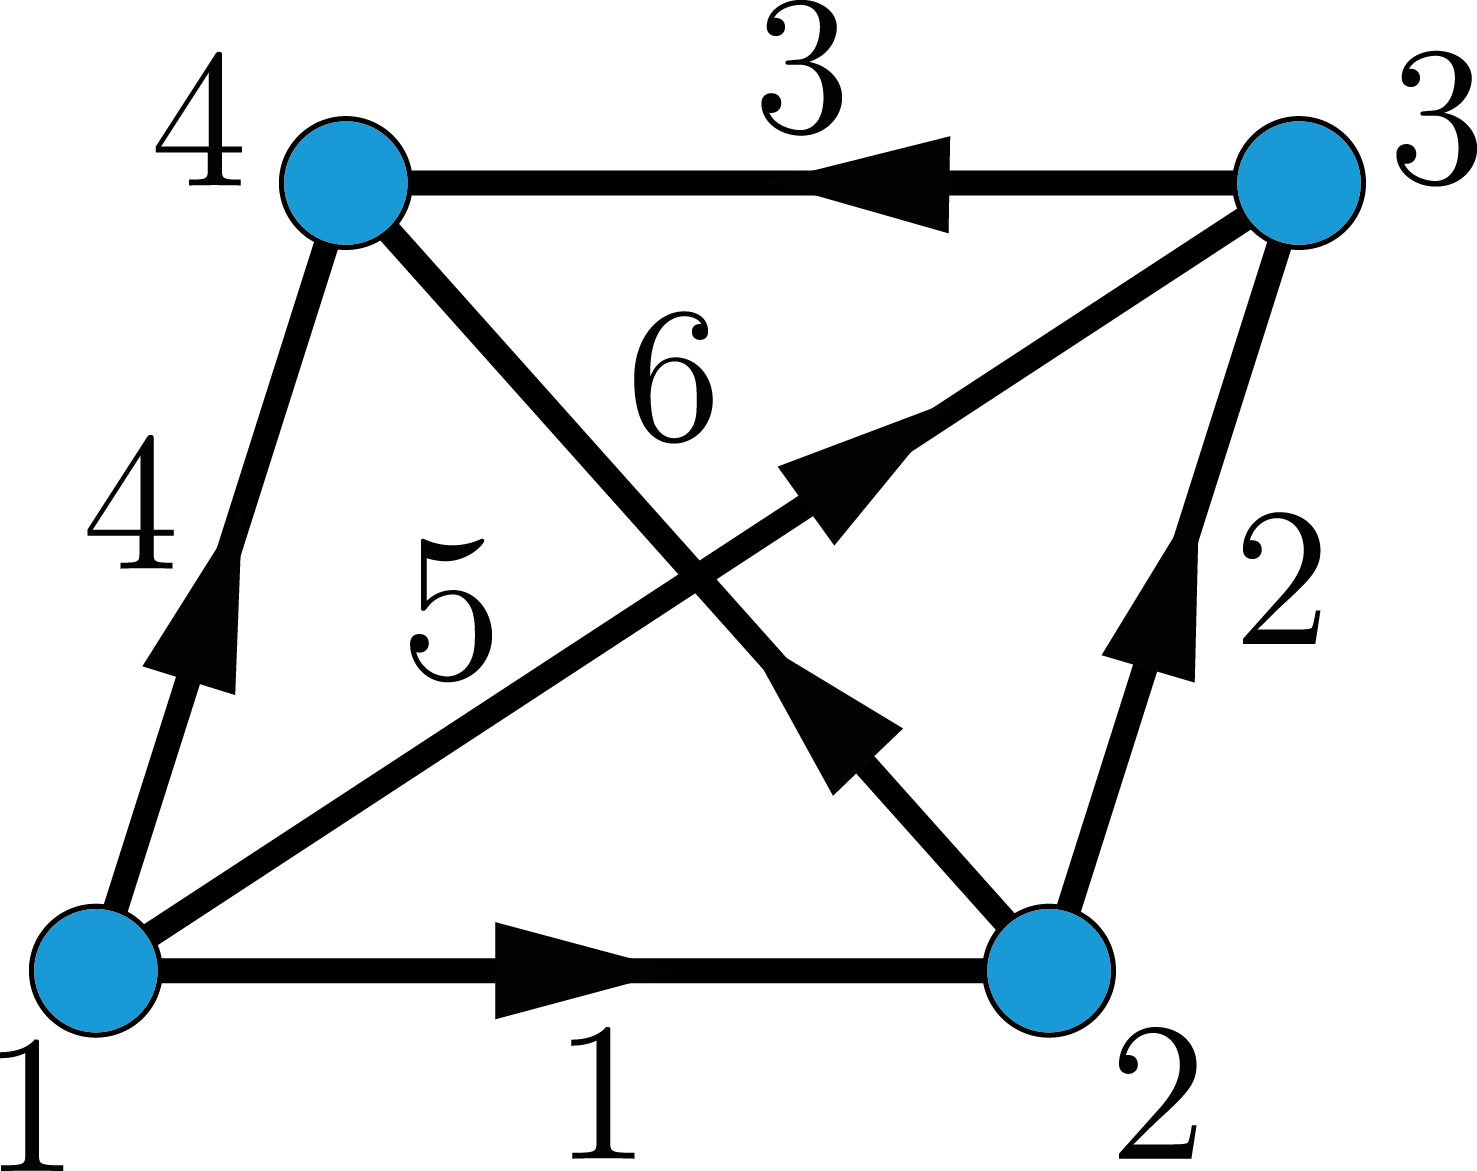
\includegraphics[width=0.2\textwidth]{./Figs/fig1}
    \caption{An example of network structure for a network of pipes}
    \label{Fig:fig1}
\end{figure}
%
%
\begin{align}
    \ket{\Delta P_\text{e}} = \mathbf{C} \ket{P_n}, \quad  \ket{q_e} = \mathbf{R} \ket{\Delta P_e}, \quad \ket{q_n} = \mathbf{C}^\top \ket{q_e} \\
    \begin{bmatrix} \Delta p_e^1 \\ \Delta p_e^2 \\\Delta p_e^3 \\\Delta p_e^4 \\\Delta p_e^5 \\ \Delta p_e^6
    \end{bmatrix} = \begin{bmatrix} 
    -1 & 1 & 0 & 0 \\
     0 & -1 & 1 & 0 \\
     0 & 0 & -1 & 1 \\
    -1 & 0 & 0 & 1 \\
    -1 & 0 & 1 & 0 \\
     0 & -1 & 0 & 1
    \end{bmatrix}\begin{bmatrix} P_n^1 \\ P_n^2 \\  P_n^3 \\P_n^4\end{bmatrix}, \quad 
    \begin{bmatrix}
    q_e^1\\    q_e^2\\    q_e^3\\    q_e^4\\    q_e^5\\    q_e^6\\
    \end{bmatrix} = \begin{bmatrix}
    R_1 & 0 & 0 & 0 & 0 & 0 \\
    0 & R_2 & 0 & 0 & 0 & 0 \\
    0 & 0 & R_3 & 0 & 0 & 0 \\
    0 & 0 & 0 & R_4 & 0 & 0 \\
    0 & 0 & 0 & 0 & R_5 & 0 \\
    0 & 0 & 0 & 0 & 0 & R_6 
    \end{bmatrix}
    \begin{bmatrix} \Delta p_e^1 \\ \Delta p_e^2 \\\Delta p_e^3 \\\Delta p_e^4 \\\Delta p_e^5 \\ \Delta p_e^6
    \end{bmatrix} \\
    \begin{bmatrix}
    q_n^1 \\    q_n^2 \\    q_n^3 \\    q_n^4 \\
    \end{bmatrix}= \begin{bmatrix} 
    -1 & 0 & 0 & -1 & -1 & 0 \\
    1 & -1 & 0 & 0 & 0 & -1 \\
    0 & 1 & -1 & 1 & 0 & 0  \\
    0 & 0 & 1 & 1 & 0 & 1
    \end{bmatrix}\begin{bmatrix}
    q_e^1\\    q_e^2\\    q_e^3\\    q_e^4\\    q_e^5\\    q_e^6\\
    \end{bmatrix}
\end{align}
